\documentclass[11pt]{article}
\usepackage{amsmath, amssymb, amscd, amsthm, amsfonts}
\usepackage{graphicx}
\graphicspath{{../plotting/}}
\usepackage{hyperref}
\usepackage{subfiles}
\usepackage{subcaption}
\usepackage{geometry}
\geometry{
 a4paper,
 total={170mm,257mm},
 left=20mm,
 top=20mm,
 }

\title{ A pendulum video and autoencoder }
\author{Pietro Sillano}

\begin{document}
\maketitle
\nocite{pytorch} 
\nocite{kchamp} 



%MAX 4 PAGINE 
%MAX 6 FIGURES
% VOLENDO INFORMAZIONI ADDIZIONALI IN APPENDICE

\section{Introduzione}
L'uso di reti neurali o deep learning per la previsione della dinamica di sistemi dinamici presenta alcune criticitá, tra cui problemi di generalizzazione al di fuori degli esempi del training set e inoltre una mancanza di interpretabilitá del modello ottenuto, dovuta al grande numero di parametri di tali modelli.

\section{Task}
L'obiettivo consiste nell' individuare un set di equazioni che possa catturare la dinamica del sistema  e che sia allo stesso tempo il piú semplice possibile.
L'idea del paper considerato consiste nel combinare un \textbf{autoencoder} che effettui una riduzione di dimensionalitá dell'input e un metodo chiamato \textbf{SINDy}(Sparse Identification of Nonlinear Dynamics) che riesce a  individuare un modello dinamico per il sistema nelle nuove coordinate latenti. \\
Infatti, non sempre i dati che vengono raccolti rappresentano la dinamica del sistema nella migliore o nella piú semplice rappresentazione possibile per cui SINDy fallirebbe o identificherebbe dei modelli con molti parametri.\\
Mentre gli autoencoder effettuano riduzioni di dimensionalitá ma non garantiscono che le nuove variabili nel latent space avranno dei modelli dinamici associati semplici.
Risulta quindi opportuna l'uso di questi due metodi simultaneamente, in modo da identificare correttamente la dinamica ma allo stesso tempo avere un modello dinamico semplice.



\section{Metodi}

\subsection{Dataset}
Il dataset considerato é una collezione di snapshot (immagini 51x51 pixel) di un video di un pendolo.
Il dataset utilizzato é generato sinteticamente(maggiori dettagli in appendice) per cui si ha una certa libertá nella creazione del dataset.\\
\begin{figure}[h]
\caption{Tre samples del dataset considerato, immagine 51 x 51 pixels.}
\centering
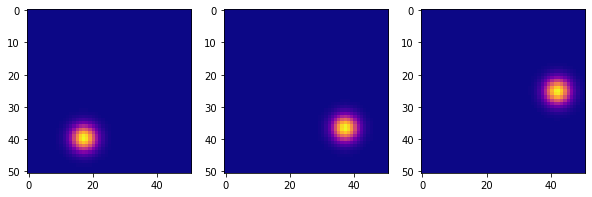
\includegraphics[width=\textwidth]{pendulum_motion}
\end{figure}%
Per generare il dataset sono state usate 100 condizioni iniziali per $\theta_0$ e 100 per $\omega_0$ combinandole assieme e escludendo le condizioni iniziali per cui la dinamica del pendolo non é un ciclo limite. Complessivamente quindi abbiamo circa 5000 condizioni iniziali differenti, per ognuna di queste abbiamo 100 snapshot e ogni snapshot é un samples con 2601(51x51) features.


\newpage
\subsection{Architettura della rete}
L'architettura utilizzata é un semplice autoencoder fully connected. L'autoencoder impara una rappresentazione non lineare dell'input in un latent space ridotto rispetto alla dimensionalitá dei samples.
L'encoder ha come input $\mathbf{x}(t) \in \mathbb{R}^n $ con $n = 2601$ e effettua una trasformazione di coordinate $\mathbf{z}(t)=\phi(\mathbf{x}(t)) \in \mathbb{R}^d$ dove d é la dimensione dello spazio latente ridotto. Mentre il decoder effettua una traformazione $\tilde{\mathbf{x}} \approx \psi(\mathbf{z})$ cercando di ricostruire l'input originario.
La rete é composta da:
\begin{itemize}
\item encoder: 3 layer fully connected da 128, 64, 32 neuroni
\item un layer nascosto formato da pochi neuroni che agisce come latent space, \item decoder: 3 layer fully connected invertiti rispetto all'encoder, quindi 32, 64, 128 neuroni.
\end{itemize}
L'architettura presentata nel paper é stata riscritta in PyTorch. \cite{pytorch}


\subsection{Sindy: Sparse Identification of Nonlinear Dynamical systems}
É un metodo di sparse regression applicato ad una libreria di possibili funzioni candidate per ricostruire la dinamica di sistemi dinamici (anche non lineari). \cite{pysindy} \\
Per costruire il modello dinamico a partire dai dati di input usiamo una libreria di funzioni e riformuliamo il problema sotto forma di regressione:

$$\dot{Z} = \mathbf{\Theta}(Z) \mathbf{\Xi}$$
La matrice $\mathbf{\Theta}(Z)$ é costruita combinando assieme funzioni candidate:
\begin{equation}
\mathbf{\Theta}(Z) =  
\begin{pmatrix}
z_1(t_0) & z_2(t_0) & z_3(t_0) & ... & sin(x_1(t_0)) & \sqrt{x_2(t_0)} & ... \\
z_1(t_1) & ... & ...  \\
 ... & ...   \\
z_1(t_f)
\end{pmatrix}
\end{equation}
Mentre la matrice incognita $\mathbf{\Xi}$ contiene i coefficienti che determinano i termini attivi della matrice theta. Idealmente vorremmo la matrice sparsa in modo da avere pochi termini selezionati dalla $\mathbf{\Theta}$.
I coefficienti $\xi$ sono aggiornati dalla rete durante il training come i pesi $\omega$ della rete.\\
\begin{equation}
\mathbf{\Xi} =  
\begin{pmatrix}
\xi_{1,1} & \xi_{1,2} & \xi_{1,3} \\ 
\xi_{2,1} & ... & ... \\
\xi_{3,1}
\end{pmatrix}
\end{equation}
Per esempio, se volessi ricostruire la dinamica del sistema unidimensionale $\dot{x} = \sin(x) $ avrei:

\begin{equation}
\dot{X} =  
\begin{pmatrix}
x(t_0) & x^2(t_0) & \sqrt{x(t_0)} & \sin(x(t_0) & ...  \\
x(t_1) & ... & ...  \\
 ... & ...   \\
x(t_f)
\end{pmatrix} 
\begin{pmatrix}
0 \\ 
0 \\
0 \\ 
1 \\ 
... \\
0
\end{pmatrix}
= 
\begin{pmatrix}
\sin(x(t_0) \\ 
\sin(x(t_1) \\
\sin(x(t_2) \\ 
... \\ 
... \\
\sin(x(t_f)
\end{pmatrix} 
= \sin(X)
\end{equation}


\subsection{Loss}
I due metodi vengono combinati tra di loro tramite la funzione di costo $L$; infatti non sará semplicemente la MSE loss (mean squared loss) tra l'input $x$ dell' autoencoder e la ricostruzione $\tilde{x}$ ma vengono aggiunti termini che garantiscono oltre alla ricostruzione dell'input, anche la ricostruzione delle derivate temporali $\dot{x}$ e $\dot{z}$ e infine un termine di regolarizzazione L1 sui coefficienti $\mathbf{\Xi} $. \\ 
Per un dataset con $m$ samples di input, ogni loss é definita come segue:

\begin{itemize}
\item $L_{recon} = \frac{1}{m}\sum_{i=1}^{m}\|x_i - \tilde{x_i}|_2^2 $  misura quanto l'autoencoder riesce a ricostruire l'input x.
\item $L_{dz} = \frac{1}{m}\sum_{i=1}^{m}\|\dot{z_i} - \Theta(z_i)\mathbf{\Xi}\|_2^2 $ misura quanto il modello predica correttamente la derivata temporale delle variabili intrinseche $z$.
\item $L_{dx} = \frac{1}{m}\sum_{i=1}^{m}\|\dot{x_i} - \dot{\tilde{x_i}}\|_2^2 $ misura quanto le predizioni di Sindy ossia $\dot{\tilde{x}}$ ricostruiscono l'input originale $\dot{x}$.
\item $L_{reg} = \frac{1}{pd}\sum_{i=1}^{pd}\|{\mathbf{\Xi}}\|_1 $ é una regolarizzazione L1 che promuove la sparsity dei coefficienti $\mathbf{\Xi}$ che coincide con identificare modelli dinamici semplici .
\end{itemize}
Per cui combinando insieme i quattro termini di loss insieme ai relativi iperparametri la loss complessiva é la seguente: 
$$L_{tot} = L_{recon} + \lambda_1L_{dx} + \lambda_2L_{dz} + \lambda_3L_{reg} $$



\section{Risultati}
Una delle difficoltá durante la model selection é la mancanza di una misura di accuratezza della dinamica individuata, pertanto ho dovuto considerare la la correttezza dei coefficienti e la parsimoniositá del modello dinamico individuato. Non tutti i modelli testati hanno identificato una dinamica plausibile. Il modello migliore ha individuato:
$$
\begin{cases} 
\dot{z_3} = 0.381 z_8 \\ 
\dot{z_8} = - 0.672 z_3
\end{cases}
$$
Dove $z_3$ e $z_8$ sono due delle variabili latenti estratte dall'autoencoder e sono le maggiormente rappresentative della dinamica.
Questo é dovuto al fatto che gli altri coefficienti erano nulli o prossimi allo zero e quindi ho potuto trascurarli. Il modello individuato non riesce a recuperare perfettamente la dinamica iniziale del pendolo ma ne cattura correttamente la dinamica in approssimazione di angoli piccoli (modello linearizzato).



\begin{figure}[h]
\centering
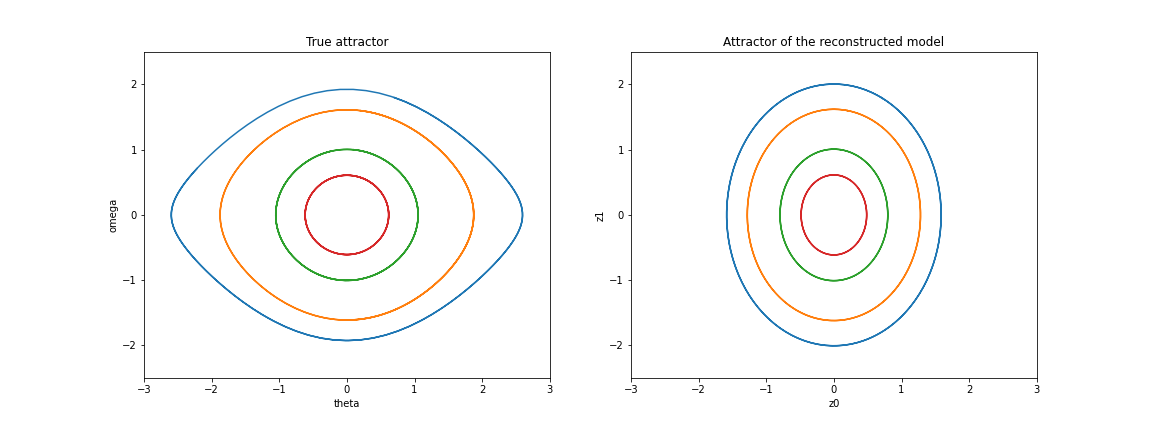
\includegraphics[width=\textwidth]{attractor}
\caption{True and reconstructed attractor}
\end{figure}

\section{Possibili sviluppi futuri}

\begin{itemize}
	\item Estendere ad altri sistemi dinamici.
	\item Utilizzare un autoencoder convoluzionale in quanto mi aspetto che le features rilevanti dell'input siano locali.
	\item Introdurre un sistema di derivate temporali al secondo ordine e  quindi provare a ricostruire direttamente $\ddot{x}$ da  $x$.
\end{itemize}



\bibliographystyle{plain}
\bibliography{bibliography.bib}
\section{Codice}
Implementazione del codice su 
\url{https://github.com/pietro-sillano/SindyPendulum}.
\newpage
\section{Appendice}
\subsection{Creazione del dataset sintetico}
Ricordando l'equazione del moto di un pendolo semplice:
$$ \ddot{\theta} = - \sin(\theta) $$
la posso riscrivere come un sistema di due ODE del primo ordine, ossia:

$$
\begin{cases} 
\dot{\theta} = \omega \\ 
\dot{\omega} = - \sin(\theta)
\end{cases}
$$
con condizioni iniziali $\theta_0$ e $\omega_0$ scelte arbitrariamente.
Ho integrato numericamente questo sistema da $t=0$ a $t=5$ con un integratore RK4 (Runge-Kutta del $4^o$ ordine) con un timestep  $dt = 0.05$.
Successivamente per generare il video del pendolo ho valutato una funzione gaussiana 2D su una griglia di 51 x 51 punti.
$$G(x,y,\theta(t)) = \exp(-A[(x - \cos{\theta(t)})^2 + (y - \sin{\theta(t)})^2])$$
In questo modo é possibile generare quanti samples sono necessari.
É importante peró variare le condizioni iniziali in modo che la rete possa avere samples del sistema in ogni punto della dinamica.


\subsection{Propagazione delle derivate temporali }
Nella funzione di loss compaiono delle derivate temporali di alcune grandezze: $\dot{x}$ assumiamo di poterla calcolare a partire dai dati di input, mentre $\dot{z}$ e $\dot{\tilde{x}}$ dobbiamo  esprimerle in funzione di grandezze note.
Per esempio, per $\dot{z}$:
\begin{itemize}
\item $m$  numero di layer nella rete,
\item $x$ =   input,
\item $z$ =   output della rete,
\item $I_j = (w_ja_{j-1} + b_j)$ valore dei neuroni layer $j$, per cui $\boxed{I_0 = (x\omega_0 + b_0)}$ e  $\boxed{z = I_m = (a_{m-1}\omega_m + b_m)}$
\item $a_{j}(I_j) = f(I_j)$ attivazione del layer l,
\end{itemize}
\begin{equation}
\frac{dz}{dt} = \frac{dI_m}{dt} = 
\frac{dI_m}{da_{m-1}}\frac{da_{m-1}}{dt}
\end{equation}

\begin{equation}
\frac{dI_m}{dt} = 
\frac{da_{m-1}}{dt} \left[\frac{d}{da_{m-1}} (a_{m-1}\omega_m + b_m)\right]
\end{equation}

\begin{equation}
\frac{dI_m}{dt} = \frac{df(I_{m-1})}{dt}  \omega_m
\end{equation}

\begin{equation}
\boxed{
\frac{dI_m}{dt} = f^\prime \frac{d(I_{m-1})}{dt}  \omega_m
}
\end{equation}%
Con condizioni al contorno date dal primo layer e dall'input:
\begin{equation}
\boxed{
\frac{dI_0}{dt} = \frac{dI_0}{dx}\frac{dx}{dt} = \dot{x} \; \omega_0
}
\end{equation}

Applicando questa regola é possibile calcolare:
\begin{itemize}
\item $\dot{z}$ conoscendo $\dot{x}$,
\item $\dot{\tilde{x}}$ conoscendo $\dot{z}$ (per quest'ultima utilizzando la relazione $\dot{z} = \Theta(z) \Xi$, essendo $z$ la grandezza nota).
\end{itemize}

\subsection{Dettagli Training}
Ho sperimentato diverse combinazioni variando la funzione di attivazione, la dimensione dello spazio latente, l'algoritmo di ottimizzazione e l'inizializzazione dei pesi. Riporto i dettagli che hanno condotto al risultato migliore:
\begin{itemize}
	\item Funzione di attivazione $f$ = ReLU per evitare fenomeni di \textbf{Vanishing Gradient}
	\item Optimizer = Adam
	\item Inizializzazione dei pesi della rete: estrazione da una distribuzione uniforme.
	\item I coefficienti $\xi$ sono stati inizializzati a $1$.
	\item Per la scelta degli iperparametri $\lambda$ nella loss function ho usato i valori indicati nel paper, rispettivamente:
$\lambda_1 = 5  \times  10^{-4},\; \lambda_2 = 5 \times 10^{-5}$. Mentre per $\lambda_3$ ho svolto alcuni test.
	\item Dimensione dello spazio latente $d = 10$.
	\item Il training é durato 1500 epoche (Early Stopping)
	\item Batch size = 1024 samples.
	\item Non ho utilizzato un validation set in quanto non aggiungeva informazioni rilevanti.
\end{itemize}

\begin{figure}
\centering
\begin{subfigure}{.3\textwidth}
    \centering
  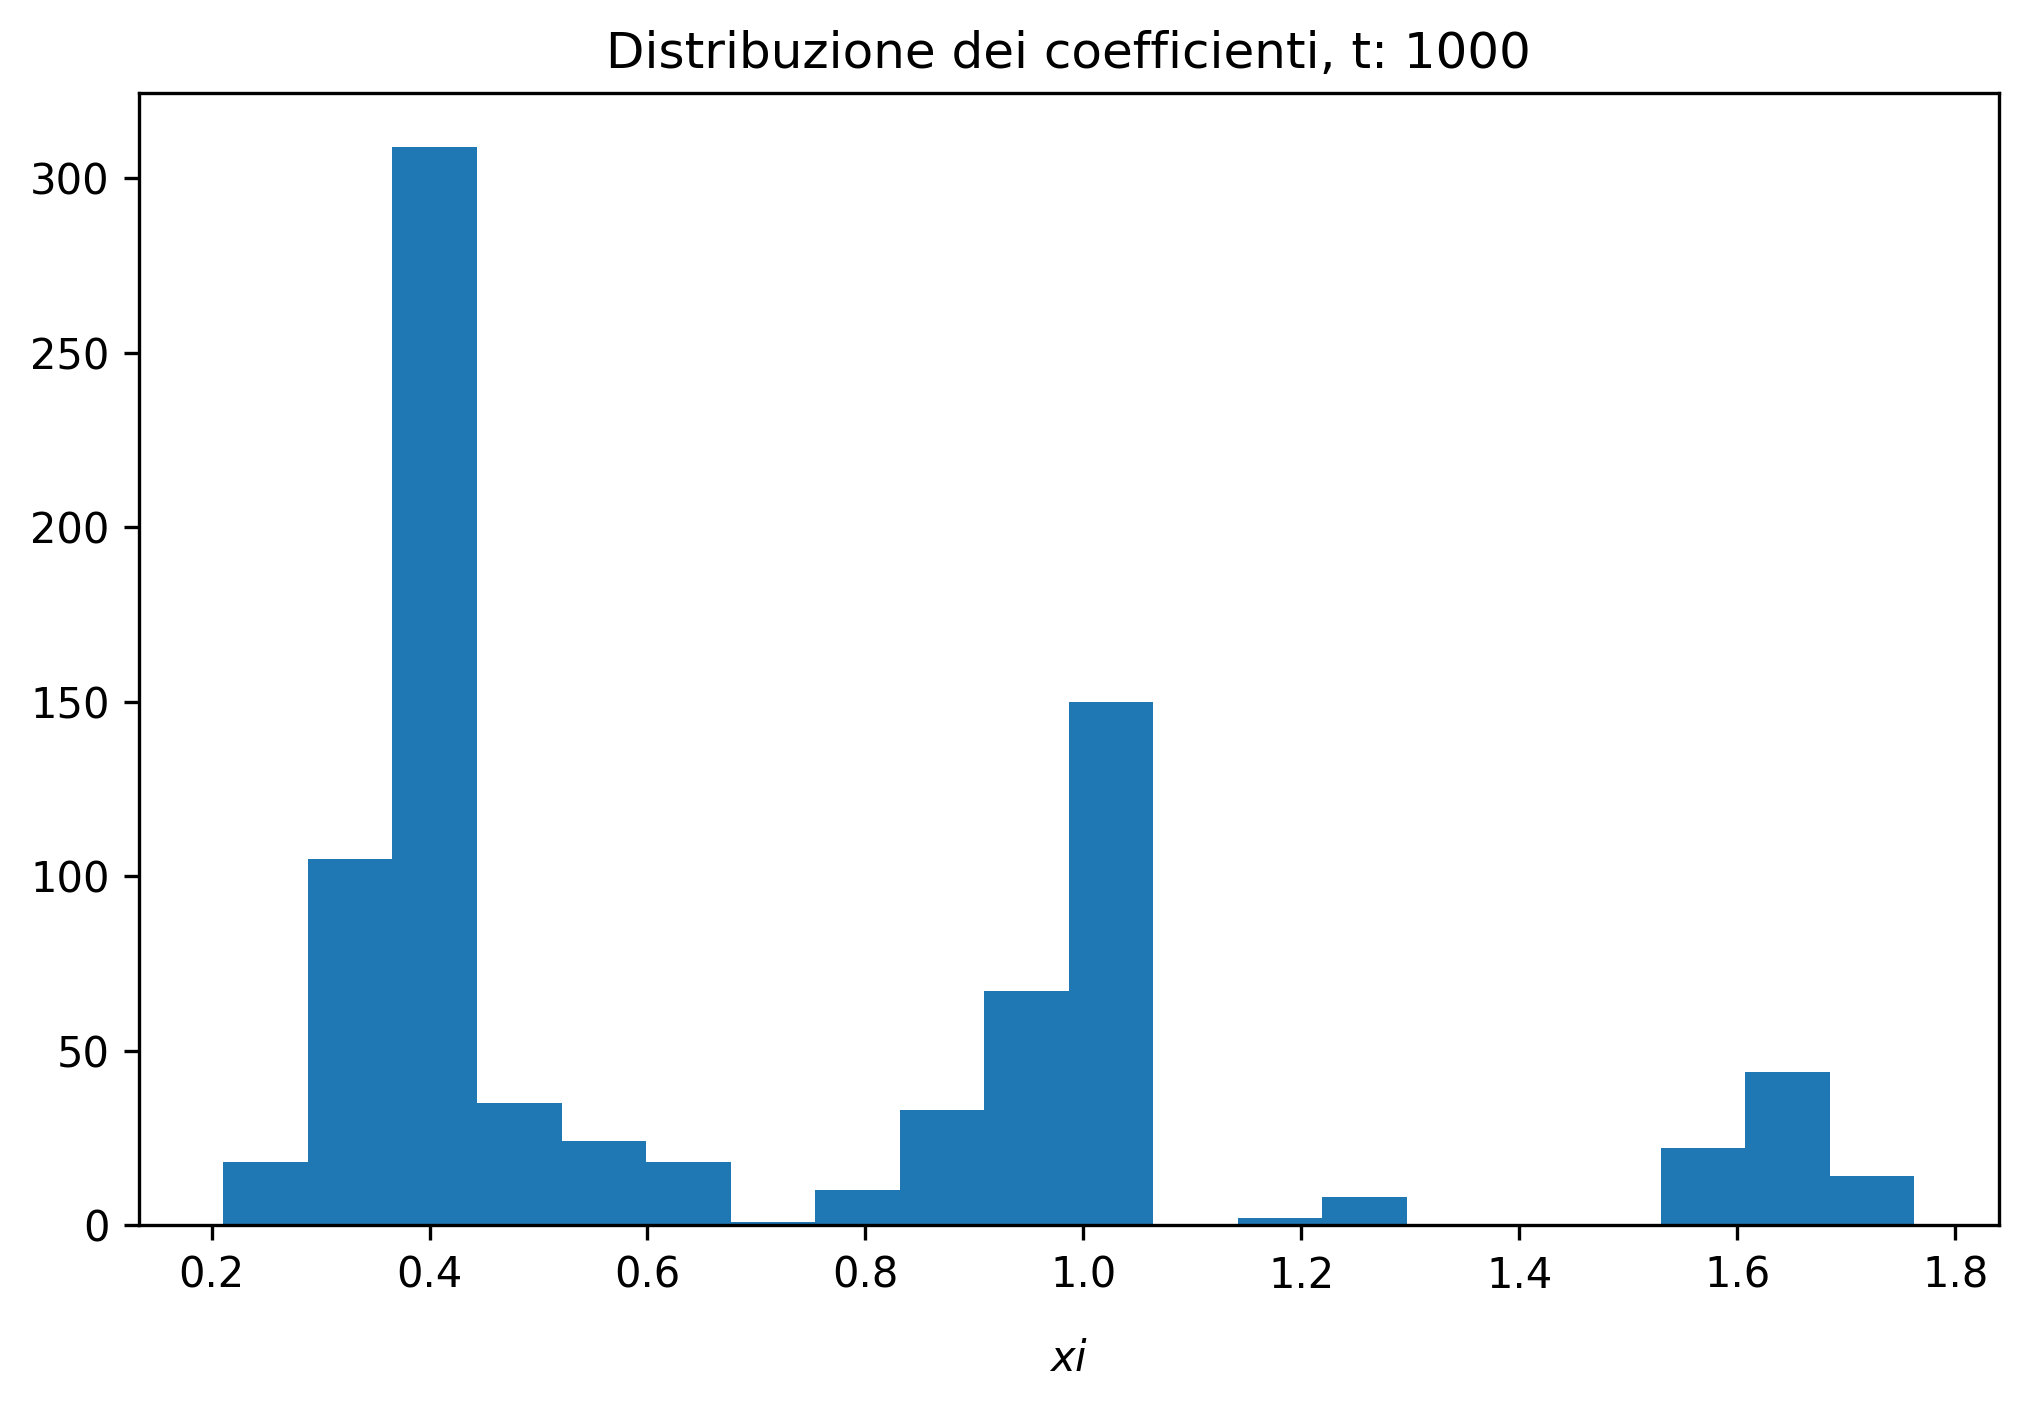
\includegraphics[width=1.\textwidth]{img/Xi_distrib_zero.png}  
%  \caption{$\lambda_3 = 0$ per cui $\Xi$ non é sparsa}
	\caption{$\lambda_3 = 0$}
\end{subfigure}
\begin{subfigure}{.3\textwidth}
    \centering
  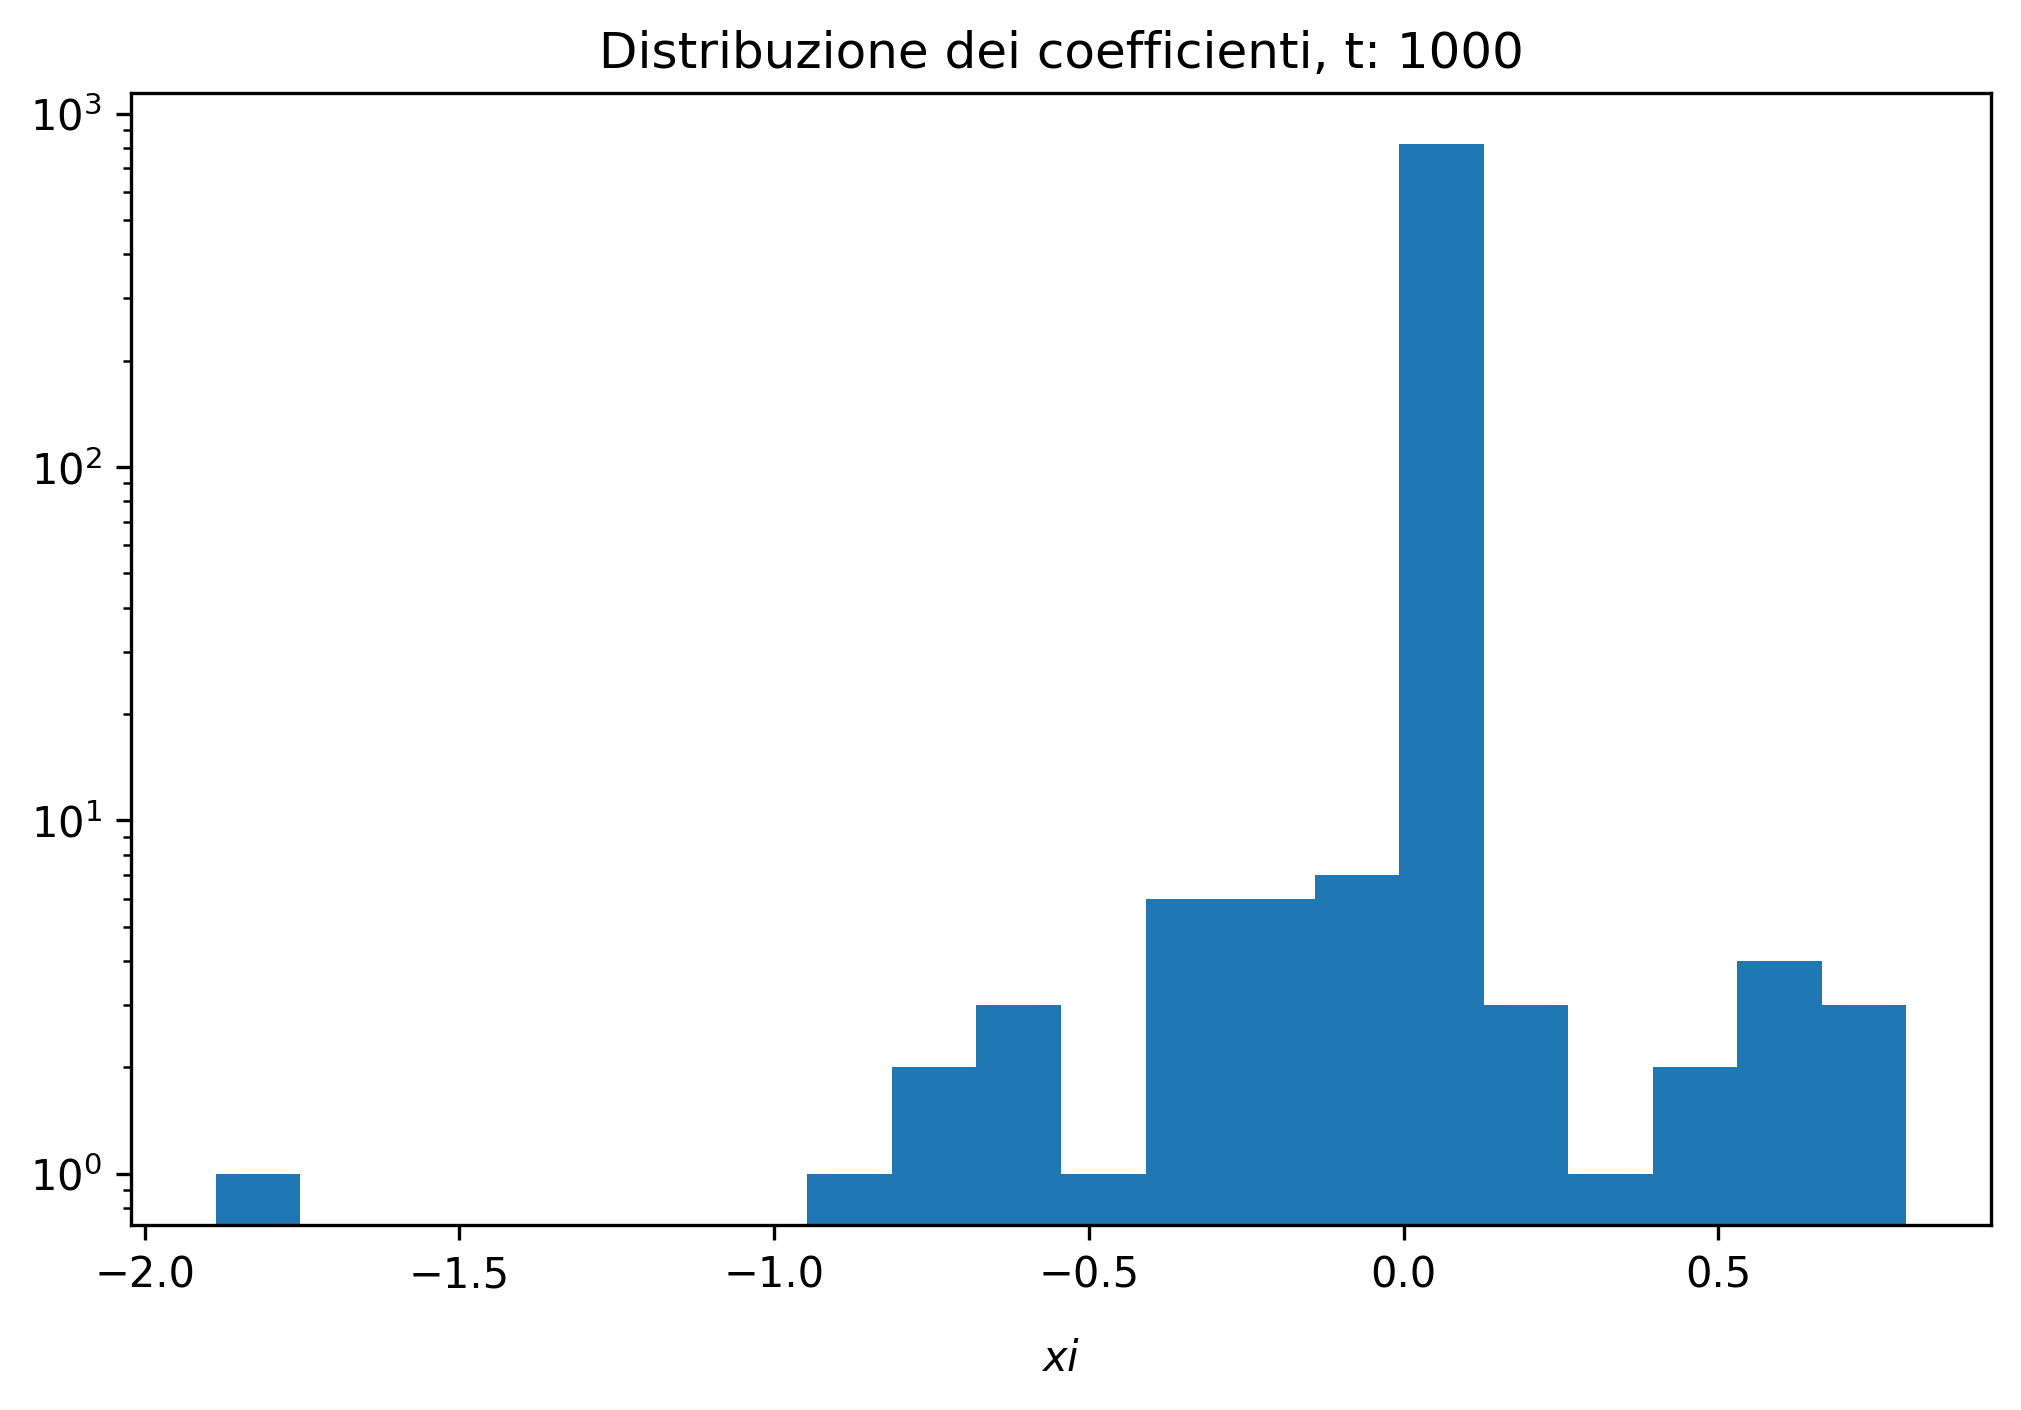
\includegraphics[width=1.\textwidth]{img/Xi_distribution_1000.png}  
  \caption{$\lambda_3 = 1 \times 10^{-5} $}
%    \caption{$\lambda_3 = 1 \times 10^{-5} $ per cui $\Xi$ é sparsa}

\end{subfigure}
\begin{subfigure}{.3\textwidth}
    \centering
  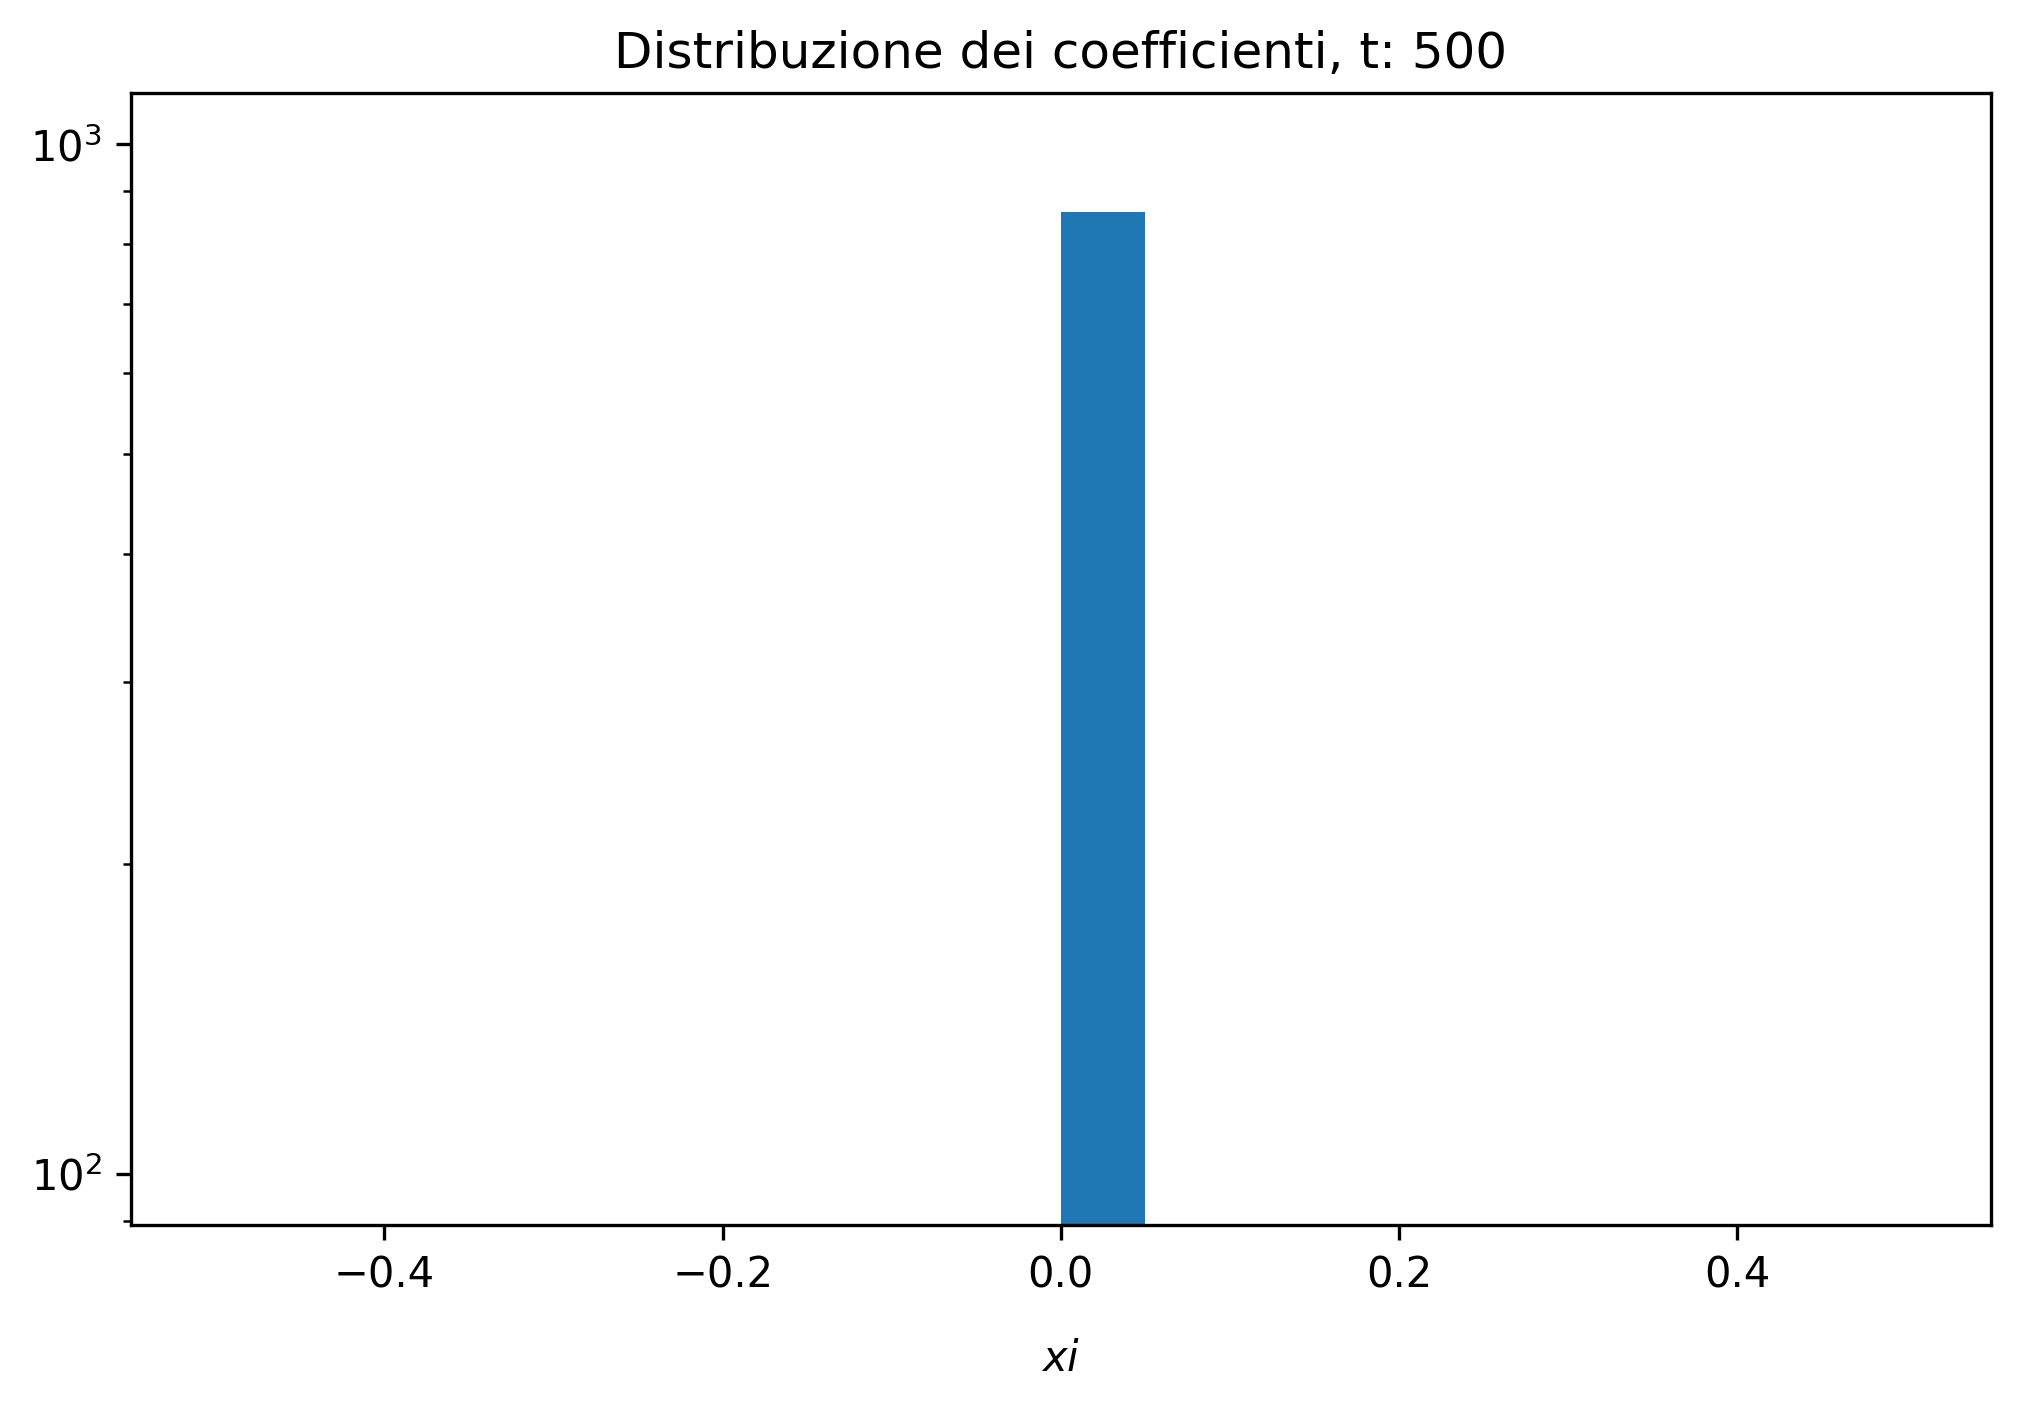
\includegraphics[width=1.\textwidth]{img/Xi_distribution_500.png}  
  \caption{$\lambda_3 = 1 \times 10^{-3} $}
%    \caption{$\lambda_3 = 1 \times 10^{-3} $ per cui  $\xi$ si annullano troppo velocemente a 500 epoche}
\end{subfigure}

\end{figure}


\begin{figure}[h]
\centering
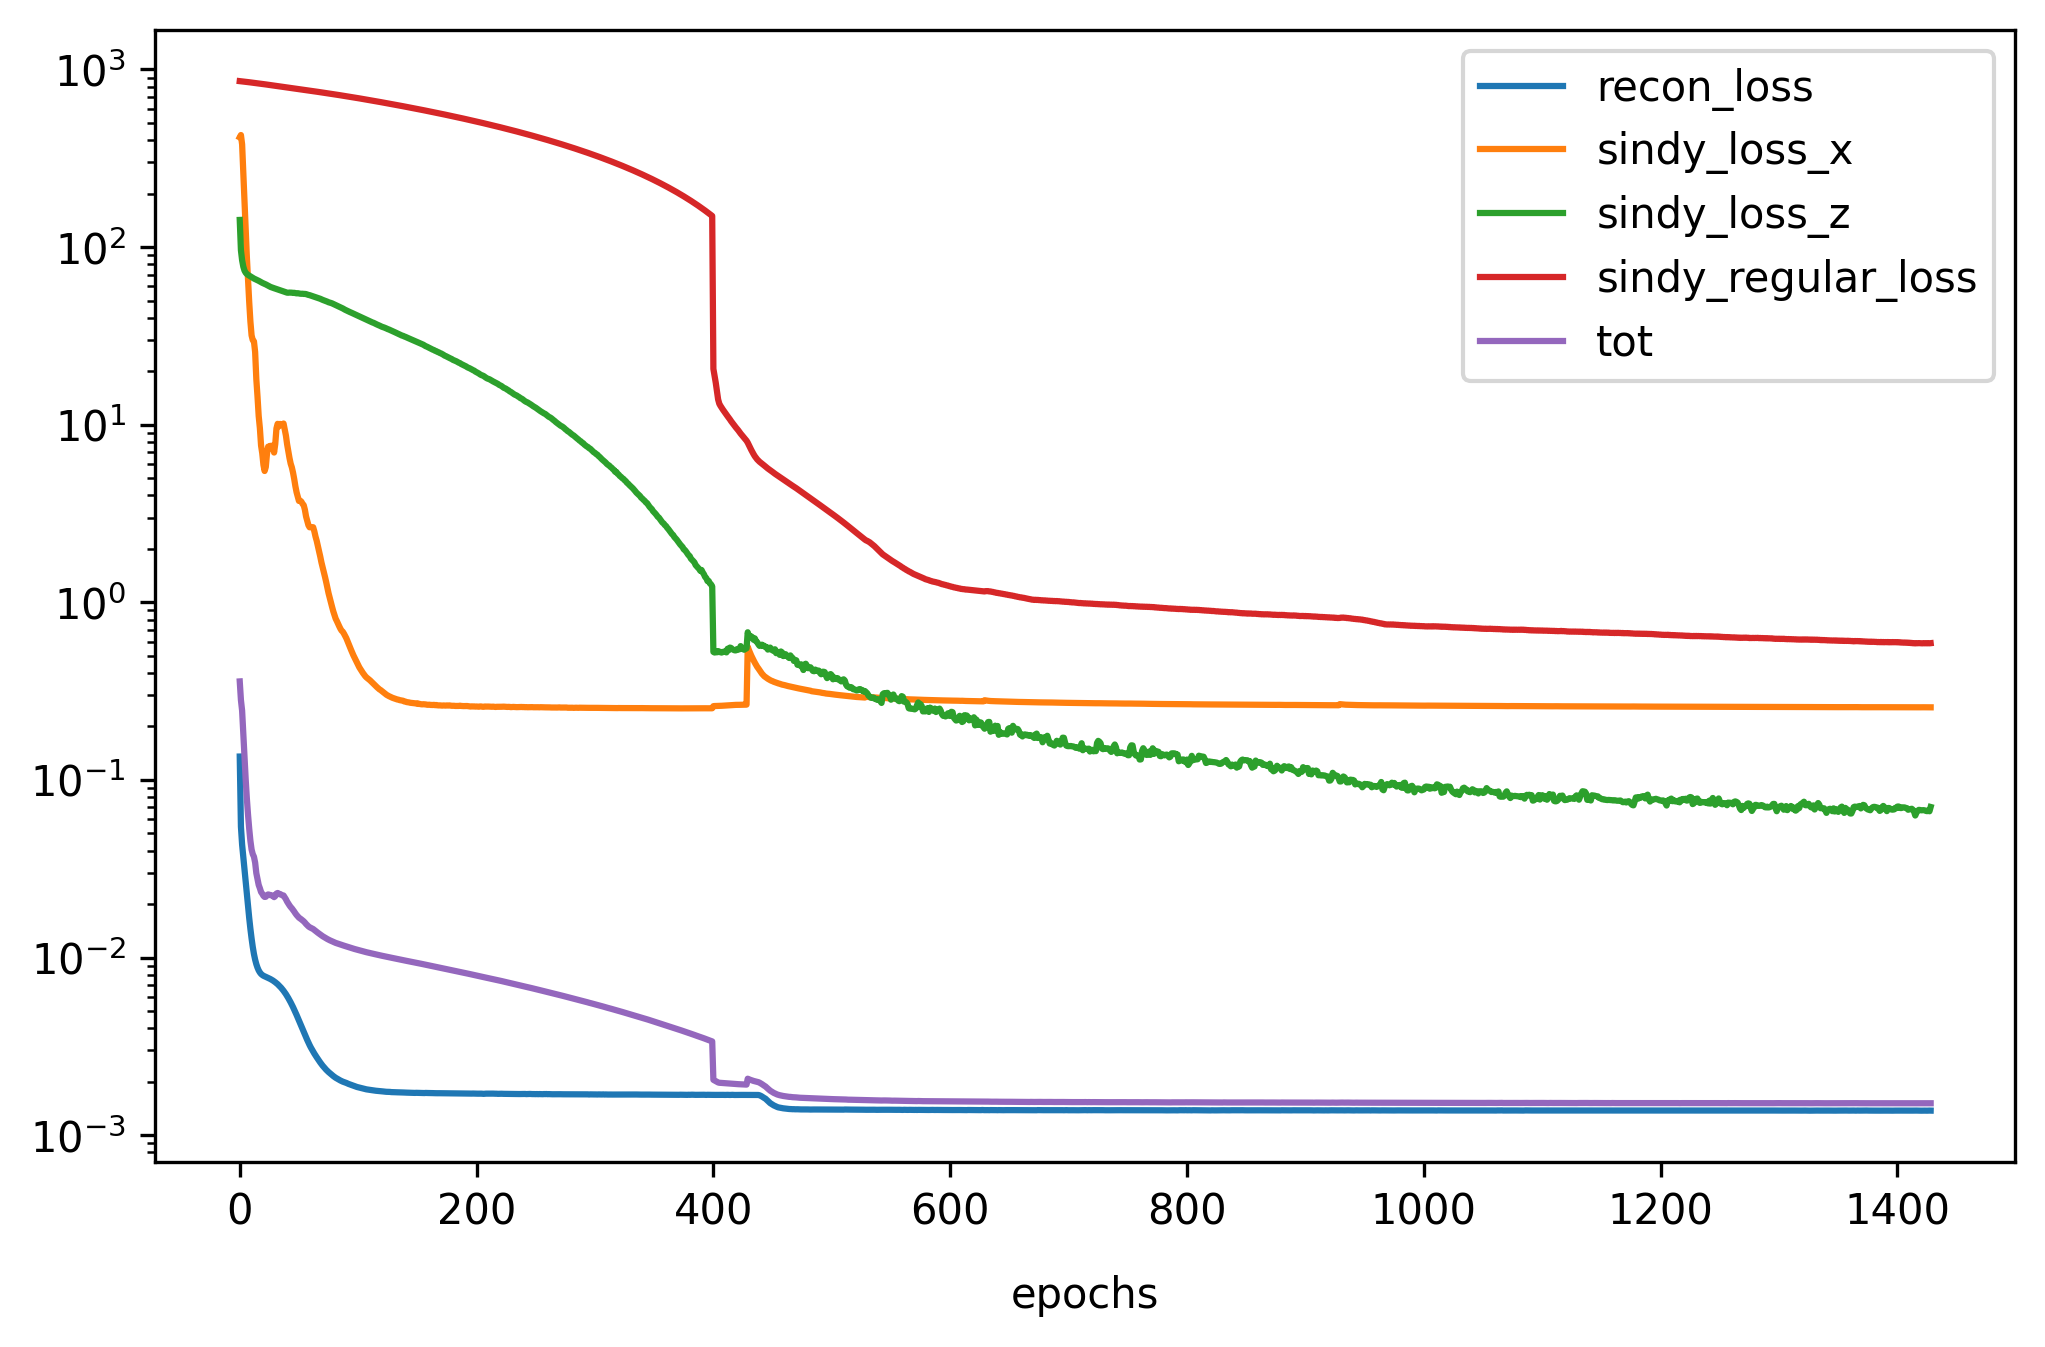
\includegraphics[width=0.8\textwidth]{img/loss.png}
\caption{Loss Functions with $\lambda_3 = 1 \times 10^{-5} $}
\end{figure}




\end{document}